\documentclass[12pt, twoside]{article}
\usepackage[letterpaper, margin=1in, headsep=0.5in]{geometry}
\usepackage[english]{babel}
\usepackage[utf8]{inputenc}
\usepackage{amsmath}
\usepackage{amsfonts}
\usepackage{amssymb}
\usepackage{tikz}
\usetikzlibrary{quotes, angles}
\usepackage{graphicx}
\usepackage{enumitem}
\usepackage{multicol}

\newif\ifmeta
\metatrue %print standards and topics tags

\title{Regents Geometry}
\author{Chris Huson}
\date{December 2021}

\usepackage{fancyhdr}
\pagestyle{fancy}
\fancyhf{}
\renewcommand{\headrulewidth}{0pt} % disable the underline of the header
\raggedbottom

\fancyhead[LE]{\thepage}
\fancyhead[RO]{\thepage \\ Name: \hspace{4cm} \,\\}
\fancyhead[LO]{BECA / Dr. Huson / Geometry 5 Congruence Transformations}

\begin{document}

\subsubsection*{5.8 Exit Note: Rotation assessment \hfill CCSS.HSG.CO.A.5}
\begin{enumerate}
\item Rotate the triangle $90^\circ$ counterclockwise around the origin, $\triangle ABC \rightarrow \triangle A'B'C'$. Complete the table of the coordinates and plot and label the image on the grid. \vspace{0.25cm}
  \begin{multicols}{2}
    $A(1,2) \rightarrow$ \\[0.7cm]
    $B(3,5) \rightarrow$ \\[0.7cm]
    $C(3,2) \rightarrow$ \\[0.7cm]
      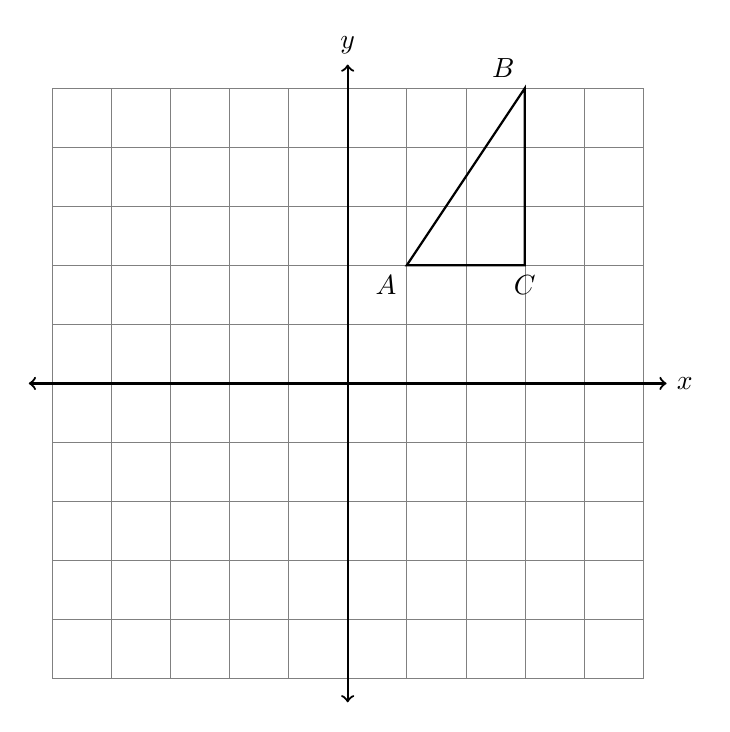
\begin{tikzpicture}[scale=.75]
      \draw [help lines] (-5,-5) grid (5,5);
      \draw [thick, <->] (-5.4,0) -- (5.4,0) node [right] {$x$};
      \draw [thick, <->] (0,-5.4)--(0,5.4) node [above] {$y$};  
      \draw [thick]
        (1,2) node[below left] {$A$}--
        (3,5) node[above left] {$B$}--
        (3,2) node[below] {$C$}--cycle;  
      \end{tikzpicture}
    \end{multicols}
  
\item $\triangle ABC$ is shown with vertices $A(0,3)$, $B(4,-1)$, and $C(5,3)$. Rotate the triangle $90^\circ$ clockwise around the origin. Write down its coordinates in a table and plot and label it on the graph.
  \begin{flushright}
  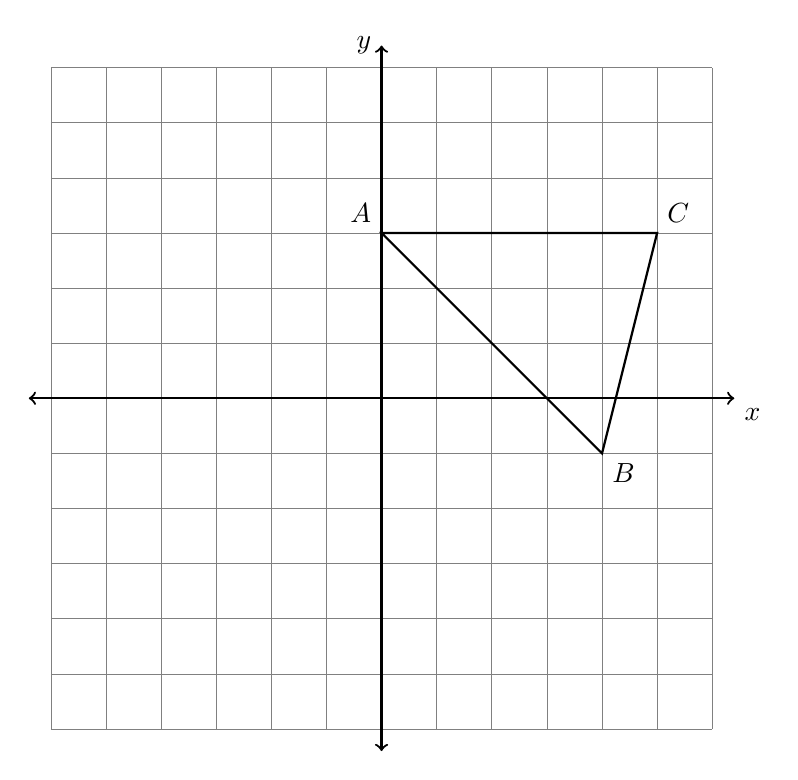
\begin{tikzpicture}[scale=0.7]
    \draw [help lines] (-6,-6) grid (6,6);
    \draw [thick, <->] (-6.4,0) -- (6.4,0) node [below right] {$x$};
    \draw [thick, <->] (0,-6.4)--(0,6.4) node [left] {$y$};
    \draw [thick] (0,3) node[above left] {$A$}--
      (4,-1) node[below right] {$B$}--
      (5,3) node[above right] {$C$}--
      cycle;
  \end{tikzpicture}
  \end{flushright}

\newpage
\subsubsection*{Challenge}
\item A rotation \emph{not} centered at the origin maps $\triangle ABC \rightarrow \triangle A'B'C'$ as shown in the diagram below. Mark the center of rotation on the grid and label it $P$. Tn the left, completely specify the transformation, including the coordinates of the center of rotation, the direction, and the magnitude in degrees.
  \begin{flushright}
  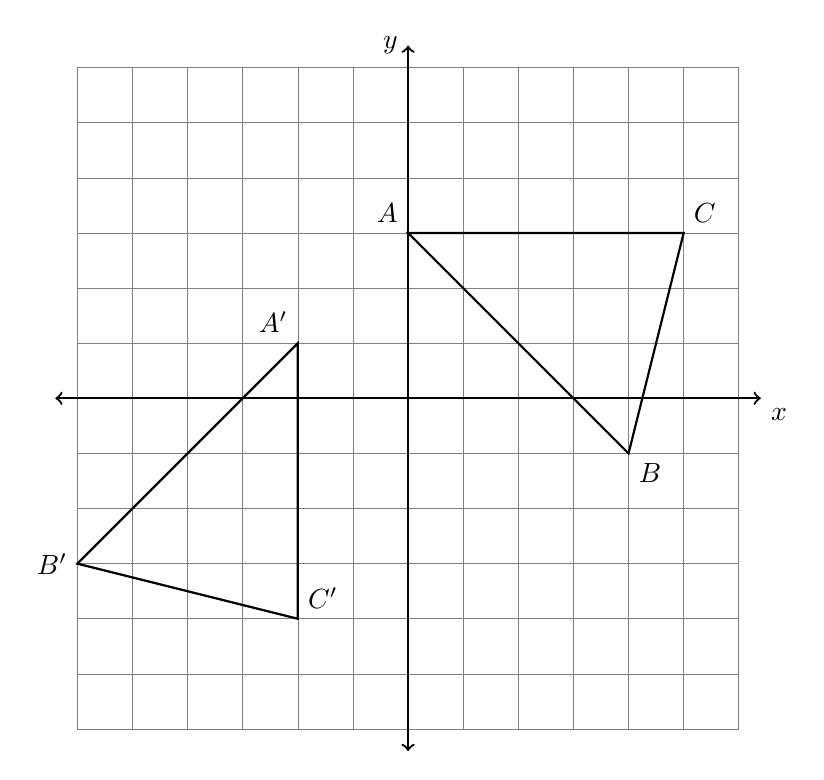
\begin{tikzpicture}[scale=0.7]
    \draw [help lines] (-6,-6) grid (6,6);
    \draw [thick, <->] (-6.4,0) -- (6.4,0) node [below right] {$x$};
    \draw [thick, <->] (0,-6.4)--(0,6.4) node [left] {$y$};
    \draw [thick] (0,3) node[above left] {$A$}--
      (4,-1) node[below right] {$B$}--
      (5,3) node[above right] {$C$}--
      cycle;
      \draw [thick] (-2,1) node[above left] {$A'$}--
      (-6,-3) node[left] {$B'$}--
      (-2,-4) node[above right] {$C'$}--
      cycle;
  \end{tikzpicture}
  \end{flushright}

\item Rotate $\triangle ABC$ $90^\circ$ counterclockwise around the point $P$. (label the image)
  \begin{center}
  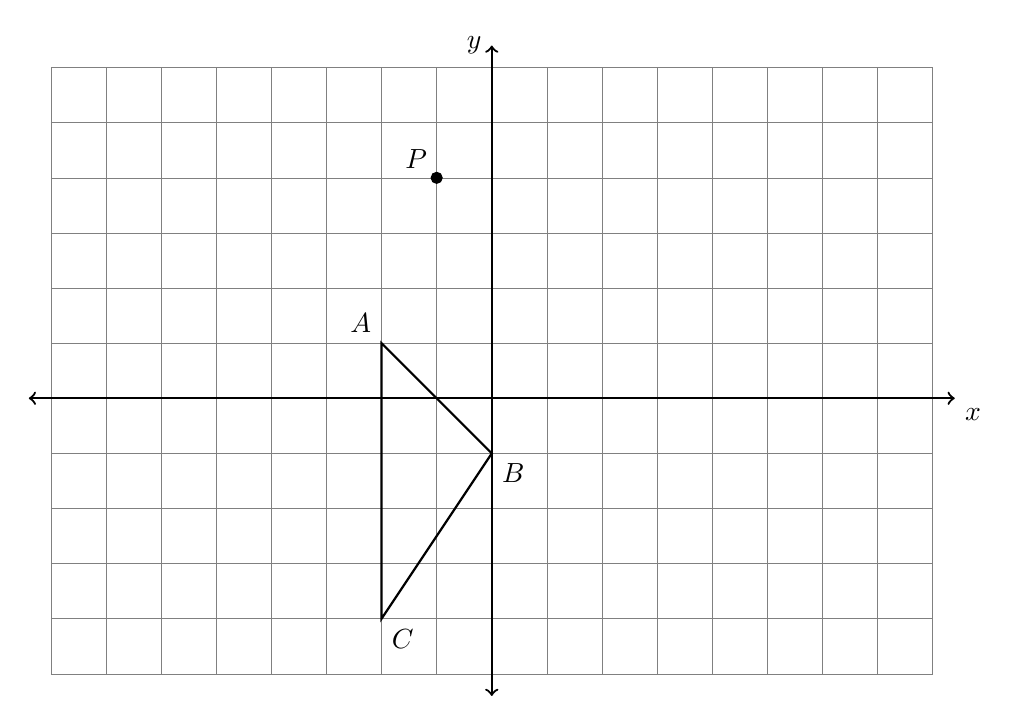
\begin{tikzpicture}[scale=0.7]
    \draw [help lines] (-8,-5) grid (8,6);
    \draw [thick, <->] (-8.4,0) -- (8.4,0) node [below right] {$x$};
    \draw [thick, <->] (0,-5.4)--(0,6.4) node [left] {$y$};
      \draw [thick] (-2,1) node[above left] {$A$}--
      (0,-1) node[below right] {$B$}--
      (-2,-4) node[below right] {$C$}--
      cycle;
      \draw[fill] (-1,4) circle [radius=0.1cm] node [above left]{$P$};
  \end{tikzpicture}
  \end{center}

\end{enumerate}
\end{document}